\begin{figure}[ht]
\centering
% Thesis-wide categorical color palette
% Usage: % Thesis-wide categorical color palette
% Usage: % Thesis-wide categorical color palette
% Usage: \input{figures/palette} in any figure file
%
% Muted primary colors -- print-friendly, visually distinct.
% Inspired by Cooper Union's red/blue primaries, softened for
% academic figures. Use palA-palC for data series in scatter
% plots, line charts, bar charts, etc.

\definecolor{palA}{HTML}{1F77B4}   % Tableau blue
\definecolor{palB}{HTML}{D62728}   % Tableau red
\definecolor{palC}{HTML}{2CA02C}   % Tableau green
 in any figure file
%
% Muted primary colors -- print-friendly, visually distinct.
% Inspired by Cooper Union's red/blue primaries, softened for
% academic figures. Use palA-palC for data series in scatter
% plots, line charts, bar charts, etc.

\definecolor{palA}{HTML}{1F77B4}   % Tableau blue
\definecolor{palB}{HTML}{D62728}   % Tableau red
\definecolor{palC}{HTML}{2CA02C}   % Tableau green
 in any figure file
%
% Muted primary colors -- print-friendly, visually distinct.
% Inspired by Cooper Union's red/blue primaries, softened for
% academic figures. Use palA-palC for data series in scatter
% plots, line charts, bar charts, etc.

\definecolor{palA}{HTML}{1F77B4}   % Tableau blue
\definecolor{palB}{HTML}{D62728}   % Tableau red
\definecolor{palC}{HTML}{2CA02C}   % Tableau green

\definecolor{nodeblue}{HTML}{B8D2E6}
\definecolor{nodeborder}{HTML}{5A87B5}
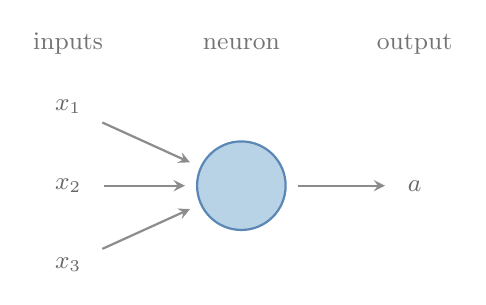
\begin{tikzpicture}[
    val/.style={font=\small, text=black!60, inner sep=2pt},
    neuron/.style={circle, draw=nodeborder, thick, fill=nodeblue,
                   minimum size=32pt, inner sep=0pt},
    conn/.style={->, thick, >=stealth, black!45},
]

% --- Input values ---
\node[val] (x1) at (-2.2, 1.0)  {$x_1$};
\node[val] (x2) at (-2.2, 0)    {$x_2$};
\node[val] (x3) at (-2.2, -1.0) {$x_3$};

% --- Neuron ---
\node[neuron] (n) at (0, 0) {};

% --- Input connections ---
\draw[conn, shorten >=4pt, shorten <=6pt] (x1) -- (n);
\draw[conn, shorten >=4pt, shorten <=6pt] (x2) -- (n);
\draw[conn, shorten >=4pt, shorten <=6pt] (x3) -- (n);

% --- Output value ---
\node[val] (out) at (2.2, 0) {$a$};
\draw[conn, shorten >=6pt, shorten <=4pt] (n) -- (out);

% --- Section labels ---
\node[val, text=black!55] at (-2.2, 1.8) {inputs};
\node[val, text=black!55] at (0, 1.8) {neuron};
\node[val, text=black!55] at (2.2, 1.8) {output};

\end{tikzpicture}
\caption{The same neuron drawn as a single unit. Each circle in
  a network diagram represents the full computation from
  \cref{fig:neuron}.}
\label{fig:neuron-abstract}
\end{figure}
